\documentclass[journal,10pt,twocolumn]{article}
\usepackage{graphicx}
\usepackage[margin=0.5in]{geometry}
\usepackage{amsmath}
\usepackage{array}
\usepackage{booktabs}
\usepackage{listings}
\providecommand{\norm}[1]{\left\lVert#1\right\rVert}
\providecommand{\abs}[1]{\left\vert#1\right\vert}
\usepackage{enumerate}
\let\vec\mathbf
\newcommand{\myvec}[1]{\ensuremath{\begin{pmatrix}#1\end{pmatrix}}}
\newcommand{\mydet}[1]{\ensuremath{\begin{vmatrix}#1\end{vmatrix}}}
\providecommand{\brak}[1]{\ensuremath{\left(#1\right)}}
\lstset{
frame=single,
breaklines=true,
columns=fullflexible
}
\title{\textbf{Matrix Assignment}}
\author{Mannava Venkatasai}
\date{September 2022}
\begin{document}
\maketitle
\paragraph{\textit{Problem Statement} - Show that the diagonals of a parallelogram divide
it into four triangles of equal area.}
\begin{enumerate}
	\item \textbf{AB=DC and AD=BC}
	\item \textbf{O is the midpoint of AC and BD}
\end{enumerate}
\begin{figure}[h]
\centering
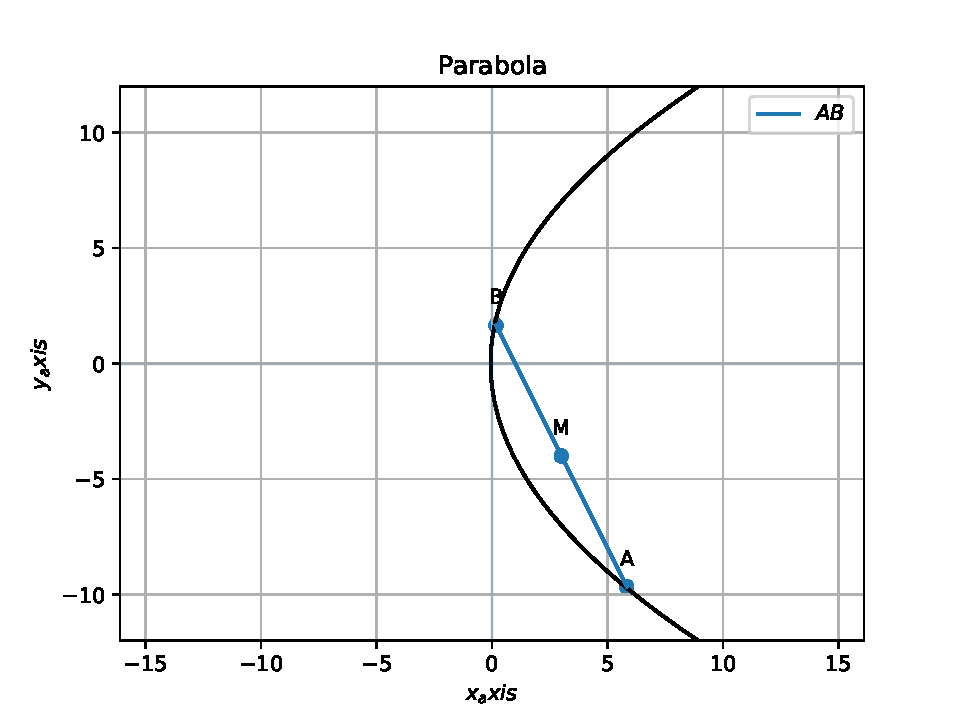
\includegraphics[width=1\columnwidth]{par.pdf}
\caption{Parallelogram ABCD With centre O}
\label{fig:Parallelogram}
\end{figure}

\section*{Solution}
\subsection*{Part 1}
\section*{Construction}
The input parameters are the lengths of AB and AD and angle between AB and ADs \vspace{2mm}\\
{
\setlength\extrarowheight{2pt}
\begin{tabular}{|c|c|c|}
	\hline
	\textbf{Symbol}&\textbf{Value}&\textbf{Description}\\
	\hline
	d&4&AB\\
	\hline
	r&3&AD\\
	\hline
	$\theta$&$\pi/6$&$\angle$A\\
	\hline
	\textbf{D}&$r%
	\begin{pmatrix}
		cos\theta\\
		sin\theta\\
	\end{pmatrix}$%
	&Point \textbf{D}\\
	\hline
	\textbf{C}&\textbf{B}+\textbf{D}
	&Point \textbf{C}\\
	\hline
\end{tabular}
}
\subsection*{Part 2}
The diagnols of a parallelogram bisect each other. 
\begin{align}
\vec{O-A} =\vec{C-O} 
\end{align}
\begin{align}
			\vec{O-D} =\vec{B-O} 
\end{align}
\begin{align}
	(\vec{C-A}) =(\vec{B-A}) + (\vec{C-B})
\end{align}
\begin{align}
	(\vec{B-D}) =(\vec{B-A}) - (\vec{C-B})
\end{align}
\begin{align}
	(\vec{O-A}) =(\vec{C-A})/2
\end{align}
\begin{align}
	(\vec{O-D}) =(\vec{B-D})/2
\end{align}
\textbf{In parallelogram ABCD} \vspace{2mm} \\
\begin{enumerate}[1.]
\item \textbf{consider $\triangle$ AOB}
\end{enumerate}
Area of triangle is given as 
\begin{align}
	\frac{1}{2}{\left | (\vec{O-A}\times\vec{B-O})\right |}
\end{align}
\begin{align}
	\frac{1}{2}{\left | (\vec{B-A})+(\vec{C-B})/2\times(\vec{B-A})-(\vec{C-B})/2\right |}
\end{align}
\begin{align}
	 \textbf{Area of $\triangle$AOB} = \frac{1}{4}{\left | (\vec{B-A})\times(\vec{C-B})\right |}
\end{align}
\vspace{5mm}
\begin{enumerate}[2.]
\item  \textbf{consider $\triangle$ BOC}
\end{enumerate}
Area of triangle is given as 
\begin{align}
	\frac{1}{2}{\left | (\vec{B-O})\times(\vec{C-O})\right |}
\end{align}
\begin{align}
	\frac{1}{2}{\left | ((\vec{B-A})-(\vec{C-B}))/2\times((\vec{B-A})+(\vec{C-B}))/2\right |}
\end{align}
\begin{align}
	\frac{1}{4}{\left | (\vec{B-A})\times(\vec{C-B})\right |}
\end{align}
\begin{align}
 \textbf{Area of $\triangle$BOC} = \frac{1}{4}{\left | (\vec{B-A})\times(\vec{C-B})\right |}
\end{align}
\vspace{5mm}
\begin{enumerate}[3.]
 \item \textbf{consider $\triangle$ COD}
\end{enumerate}
Area of triangle is given as \\
\begin{align}
	\frac{1}{2}{\left |(\vec{C-O})\times(\vec{D-O})\right |}
\end{align}
\begin{align}
	\frac{1}{4}{\left | (\vec{B-A})\times(\vec{C-B})\right |}
\end{align}
\begin{align}
\textbf{Area of $\triangle$COD} = \frac{1}{4}{\left | (\vec{B-A})\times(\vec{C-B})\right |}
\end{align}
\vspace{5mm}
\begin{enumerate}[4.]
\item \textbf{consider $\triangle$ DOA}
\end{enumerate}
Area of triangle is given as \\
\begin{align}
	\frac{1}{2}{\left |( \vec{A-O})\times(\vec{D-O})\right |}
\end{align}
\begin{align}
	\frac{1}{2}{\left | (-(\vec{B-A})-(\vec{C-B}))/2\times(-(\vec{B-A})+(\vec{C-B}))/2\right |}
\end{align}
\begin{align}
	\frac{1}{4}{\left | (\vec{B-A})\times(\vec{C-B})\right |}
\end{align}
\begin{align}
\textbf{Area of $\triangle$AOD} = \frac{1}{4}{\left | (\vec{B-A})\times(\vec{C-B})\right |}
\end{align}
Hence from the above results we can conclude that \vspace{3mm} \\
\textbf{ar($\triangle${AOB})=ar($\triangle${BOC})=ar($\triangle${COD})=ar($\triangle${DOA})\\= 1/4*${\left | \textbf{B-A}\times\textbf{C-B}\right |}$}  \vspace{4mm} \\
\textbf{Hence We prooved that the diagonals of a parallelogram divide it into 
four triangles of equal area.} \vspace{4mm} \\
\end{document}
